%% if you are submitting an initial manuscript then you should have submission as an option here
%% if you are submitting a revised manuscript then you should have revision as an option here
%% otherwise options taken by the article class will be accepted
\documentclass[submission]{FPSAC2023}
%% but DO NOT pass any options (or change anything else anywhere) which alters page size / layout / font size etc

%% note that the class file already loads {amsmath, amsthm, amssymb}

\usepackage{graphicx}
\usepackage{listings}
\usepackage{lineno}
%\usepackage[margin=3cm]{geometry}
\usepackage[all,cmtip, color,matrix,arrow]{xy}
\usepackage{subfig}

\usepackage{comment}
\usepackage{hyperref}
\usepackage[capitalize]{cleveref}  
\crefname{thm}{Theorem}{Theorems}
\usepackage{bbold}
\usepackage[export]{adjustbox}
%\usepackage{tikz-cd}
%\usepackage{xr}
%\usetikzlibrary{babel}
\usepackage{todonotes}
\usepackage{bm}
\usepackage{wrapfig}
\usepackage{bbold}
\usepackage{float}
\usepackage{mathtools}
\usepackage{aliascnt}
\newaliascnt{eqfloat}{equation}
\newfloat{eqfloat}{h}{eqflts}
\floatname{eqfloat}{Equation}
\usepackage{dirtytalk}

\newcommand*{\ORGeqfloat}{}
\let\ORGeqfloat\eqfloat
\def\eqfloat{%
  \let\ORIGINALcaption\caption
  \def\caption{%
    \addtocounter{equation}{-1}%
    \ORIGINALcaption
  }%
  \ORGeqfloat
}
\newcommand{\raul}[1]{\todo[color=green!30,inline]{CH, #1}}

\newcommand{\yannic}[1]{\todo[color=violet!30,inline]{YV, #1}}

\theoremstyle{definition}
\newtheorem{thm}{Theorem}[section]
\newtheorem{prop}[thm]{Proposition}
\newtheorem{lm}[thm]{Lemma}
\newtheorem{cor}[thm]{Corollary}
\newtheorem{obs}[thm]{Observation}
\newtheorem{defin}[thm]{Definition}
\newtheorem{smpl}[thm]{Example}
\newtheorem{quest}[thm]{Question}
\newtheorem{prob}[thm]{Problem}
\newtheorem{conj}[thm]{Conjecture}
\newtheorem{rem}[thm]{Remark}
\crefname{lm}{Lemma}{Lemmas}
\crefname{thm}{Theorem}{Theorems}
\crefname{prop}{Proposition}{Propositions}
\crefname{defin}{Definition}{Definitions}
\crefname{rem}{Remark}{Remarks}

\newcommand{\oPi}{\mathbf{C}}
\newcommand{\opi}{\vec{\boldsymbol{\pi}}}
\newcommand{\otau}{\vec{\boldsymbol{\tau}}}
\newcommand{\olambda}{\vec{\boldsymbol{\gamma}}}
\newcommand{\msum}{\sideset{^M}{}\sum}
\newcommand{\nestohedra}{nestohedra}
\newcommand{\gpHa}{\mathbf{GP}}
\newcommand{\gHa}{\mathbf{G}}
\newcommand{\citestan}{\cite[Proposition 3.2]{gebhard99}}
\newcommand{\parpi}{\boldsymbol{\pi}}
\newcommand{\partau}{\boldsymbol{\tau}}
\newcommand{\makepar}{\boldsymbol{\lambda}}
\newcommand{\uhsm}{\boldsymbol{\Psi}}
\newcommand{\uHsm}{\boldsymbol{\Psi}}
\newcommand{\sqbinom}{\genfrac{[}{]}{0pt}{}}


\newcommand{\bfpsigrf}{$\mathbf{\Psi}_{\mathbf{Q}}$}

\newcommand{\pper}{marked permutation }
\newcommand{\ppers}{marked permutations }
\newcommand{\pperp}{marked permutation.}
\newcommand{\ppersp}{marked permutations.}

\newcommand{\stirling}[2]{\genfrac{[}{]}{0pt}{}{#1}{#2}}%binomial coefficients
\newcommand{\III}{\vec{\mathbf{I}}}
\newcommand{\JJJ}{\vec{\mathbf{J}}}


\DeclareMathOperator{\w}{\mathcal{W}}
\DeclareMathOperator{\pos}{\mathrm{pos}}
\DeclareMathOperator{\s}{\mathrm{mset}}
\DeclareMathOperator{\ms}{\mathrm{mset}}
\DeclareMathOperator{\Alg}{\mathrm{Alg}}
\DeclareMathOperator{\im}{im}
\DeclareMathOperator{\id}{id}
\DeclareMathOperator{\comu}{comu}
\DeclareMathOperator{\rest}{\mathbf{res}}
\DeclareMathOperator{\Orth}{Orth}
\DeclareMathOperator{\cano}{cano}
\DeclareMathOperator{\Ppatp}{\mathbf{Ppat}^*}
\DeclareMathOperator{\dpt}{\mathbf{depth}}
\DeclareMathOperator{\pat}{\mathbf{pat}}
\DeclareMathOperator{\Pat}{\mathrm{Pat}}
\DeclareMathOperator{\Func}{\mathrm{Func}}
\DeclareMathOperator{\spn}{\mathrm{span}}
\DeclareMathOperator{\inc}{\mathrm{inc}}
\DeclareMathOperator{\Ch}{\mathrm{Ch}}
\DeclareMathOperator{\tvs}{\textvisiblespace}
\DeclareMathOperator{\sFunc}{\mathrm{SurFunc}}
\DeclareMathOperator{\End}{\mathrm{End}}
%\usepackage{lipsum}

\newcommand{\bfa}{\mathbf{a}}

%combinatorial concepts
\newcommand{\Sr}{\mathrm{S}} %symmetric group
\newcommand{\opp}[1]{\overline{#1}} %for opposite
\newcommand{\len}{l} % for length (degree) of a composition or partition
%\newcommand{\maxflat}{\hat{1}}
\newcommand{\maxflat}{\widehat{I}}
\newcommand{\minflat}{\{I\}}
\newcommand{\ifac}{
\begin{picture}(3,5)(0,0)
\put(0,0){\textup{!}}\put(1.5,4.8){\circle{3}}
\end{picture}
} %cyclic factorial
\newcommand{\acyc}[1]{#1 !} %acyclic orientations

%linear operators


%categories
\newcommand{\Fset}{\mathsf{Set^{\times}}}
\newcommand{\Veck}{\mathsf{Vec}_\Kb} 
\newcommand{\Vect}{\mathsf{Vect}}
\newcommand{\gVec}{\mathsf{gVec}}
\newcommand{\Set}{\mathsf{Set}}
\newcommand{\Ss}{\mathsf{Sp}} % set species
\newcommand{\Ssk}{\mathsf{Sp}_\Kb} %vector species
\newcommand{\Spr}{\mathsf{Spr}} % set species with restrictions

\newcommand{\Mo}[1]{\mathsf{Mon}(#1)} %monoids
\newcommand{\Co}[1]{\mathsf{Comon}(#1)} %comonoids
\newcommand{\Bo}[1]{\mathsf{Bimon}(#1)} %bimonoids
\newcommand{\Kb}{\mathbb{K}} 



%generic set species
\newcommand{\rP}{\mathrm{P}}
\newcommand{\rQ}{\mathrm{Q}}
\newcommand{\rH}{\mathrm{H}}
\newcommand{\rR}{\mathrm{R}}


%generic species with restrictions
\newcommand{\prP}{\mathtt{P}}
\newcommand{\prQ}{\mathtt{Q}}
\newcommand{\prH}{\mathtt{H}}
\newcommand{\prR}{\mathtt{R}}


%set species
\newcommand{\rE}{\mathrm{E}}
\newcommand{\rL}{\mathrm{L}}
%\newcommand{\rX}{\mathrm{X}}
\let\rPi=\Pi %flats
\let\rSig=\Sigma
\newcommand{\rSigh}{\widehat{\rSig}} %decompositions = weak compositions
\newcommand{\rG}{\mathrm{G}} %graphs
\newcommand{\rGP}{\mathrm{GP}} %generalized permutahedra
\newcommand{\SP}{\mathfrak{p}} %standard permutahedron

%generic species
\newcommand{\thh}{\mathbf{h}} 
\newcommand{\tg}{\mathbf{g}}
\newcommand{\tk}{\mathbf{k}}
\newcommand{\tp}{\mathbf{p}} 
\newcommand{\tq}{\mathbf{q}}
\newcommand{\tr}{\mathbf{r}}
\newcommand{\ta}{\mathbf{a}}
\newcommand{\tb}{\mathbf{b}} 
\newcommand{\tc}{\mathbf{c}}
\newcommand{\td}{\mathbf{d}}
\newcommand{\trr}{\mathbf{r}} 
\newcommand{\tm}{\mathbf{m}} %module
\newcommand{\brac}{\nu} %Lie bracket

%examples of species
\newcommand{\tone}{\mathbf{1}}
\newcommand{\wU}{\mathbf{U}}
\newcommand{\wX}{\mathbf{X}}
\newcommand{\wE}{\mathbf{E}} %exponential species
\newcommand{\wL}{\mathbf{L}} %linear orders
\newcommand{\wI}{\mathbf{I}}%used in macro \tLL
\newcommand{\tLL}{\wI\hspace*{-2pt}\wL} %pairs of chambers
\newcommand{\tLie}{\mathbf{Lie}} %Lie species
\newcommand{\tPi}{\mathbf{\Pi}} %flats
\newcommand{\tSig}{\mathbf{\Sigma}} %faces
\newcommand{\tSigh}{\mathbf{\widehat{\Sigma}}} % decompositions
\newcommand{\te}{\mathbf{e}} %elements
\newcommand{\tG}{\mathbf{G}} %graphs
\newcommand{\tcG}{\mathbf{cG}} %connected graphs
\newcommand{\tGP}{\mathbf{GP}} 

%some isomorphisms
\let\isoflat=\psi
\let\isolinear=\psi
\let\isograph=\varphi


%Fock functors
\newcommand{\contra}[1]{#1^{\vee}} 
\newcommand{\Kc}{\mathcal{K}}
\newcommand{\Kcb}{\overline{\Kc}}
\newcommand{\cKc}{\contra{\Kc}}
\newcommand{\cKcb}{\contra{\Kcb}}

%functors
\newcommand{\Tc}{\mathcal{T}}
\newcommand{\Tcq}{\Tc_q}
\newcommand{\Sc}{\mathcal{S}}
\newcommand{\Pc}{\mathcal{P}} %primitive element functor
\newcommand{\Qc}{\mathcal{Q}} %indecomposables
\newcommand{\Uc}{\mathcal{U}} %universal enveloping algebra

\newcommand{\sq}{{{\scriptstyle{\square}}}}

%objects
\newcommand{\xx}{\mathrm{x}}
\newcommand{\yy}{\mathrm{y}}
\newcommand{\zz}{\mathrm{z}}
%\usepackage{amsaddr}

\usepackage{lipsum}

%% define your title in the usual way
\title[Pattern Hopf algebras, antipode and reciprocity]{Pattern Hopf algebras, antipode and reciprocity}

%% define your authors in the usual way
%% use \addressmark{1}, \addressmark{2} etc for the institutions, and use \thanks{} for contact details
\author[R. Penaguiao, Y. Vargas]{Raul Penaguiao\thanks{\href{mailto:raul.penaguiao@mis.mpg.de}{raul.penaguiao@mis.mpg.de} Work of Penaguiao is partially supported by SNF grant P2ZHP2
19130} \addressmark{1}, Yannic Vargas \thanks{\href{mailto:yvargaslozada@tugraz.at}{yvargaslozada@tugraz.at} Work of Vargas is supported by  Austrian Science Fund FWF, grant I 5788 PAGCAP.} \addressmark{2}}


%% then use \addressmark to match authors to institutions here
\address{\addressmark{1} Max Planck Institute for Mathematics in the Sciences, Leipzig \\ \addressmark{2} Technische Universität Graz}

%% put the date of submission here
\received{\today}

%% leave this blank until submitting a revised version
%\revised{}

%% put your English abstract here, or comment this out if you don't have one yet
%% please don't use custom commands in your abstract / resume, as these will be displayed online
%% likewise for citations -- please don't use \cite, and instead write out your citation as something like (author year)
\abstract{
The permutation pattern Hopf algebra is a commutative filtered and connected Hopf algebra.
Its product structure stems from counting patterns of a permutation.
The Hopf algebra was shown to be a free commutative algebra and to fit into a general framework of pattern Hopf algebras, via species with restrictions. In this work we introduce the cancellation-free and grouping-free formula for the antipode of the permutation pattern Hopf algebra, via the sign-reversing involution method.
This formula has applications on polynomial invariants on permutations, in particular for obtaining reciprocity theorems.
In fact, we study a brand new polynomial invariant on permutations amenable to this method.
On our way, we also introduce the packed word patterns Hopf algebra and present a formula for its antipode. 
Species in parking functions are also introduced.
}

%% put your French abstract here, or comment this out if you don't have one
%\resume{À faire.}

%% put your keywords here, or comment this out if you don't have them yet
\keywords{permutations, presheaves, species with restrictions, species, Hopf algebras, free algebras, antipode, cancellation-free, chromatic, reciprocity.}

%% you can include your bibliography however you want, but using an external .bib file is STRONGLY RECOMMENDED and will make the editor's life much easier
%% regardless of how you do it, please use numerical citations; i.e., [xx, yy] in the text

%% this sample uses biblatex, which (among other things) takes care of URLs in a more flexible way than bibtex
%% but you can use bibtex if you want
\usepackage[backend=bibtex]{biblatex}
\addbibresource{sample.bib}
%% note the \printbibliography command at the end of the file which goes with these biblatex commands

\begin{document}

\maketitle
%% note that you DO NOT have to put your abstract here -- it is generated by \maketitle and the \abstract and \resume commands above

%\tableofcontents

This is a shorter version of the preprint \cite{PV2022} that is currently submitted to a journal. Many proofs and details omitted here can be found in \cite{PV2022}.

\section{Introduction}
In his now celebrated  ``Lemma 14'', Takeuchi (see \cite{Takeuchi1971}, Lemma 14) obtained a quite general formula for the antipode of a Hopf algebra. 
This is an antipode formula for any filtered Hopf algebra, which can be applied in much generality and fits the framework of \textbf{pattern Hopf algebras}, introduced in \cite{Penaguiao2020}.
However, it has been observed that it is not the most economical formula, as it leaves some cancellations to be made.


Economical formulas for antipodes in Hopf algebras in combinatorics have played an important role in extracting old and new combinatorial equations, see \cite{aguiar2017hopf, BS2017, humpert2012incidence, Schmitt1993, xu2022cancellation}.
In particular, with such a formula, Humpert and Martin were able to explain, in \cite{humpert2012incidence}, an elusive \textit{reciprocity relation} on graphs first presented by Stanley in \cite{stanley1975combinatorial}.
A method for obtaining a cancellation-free formula that seem to work with a large family of Hopf algebras was brought forth by Sagan and Benedetti in \cite{BS2017}, called \textit{sign-reversing involution method}, which we leverage here.
%This is a classical method in enumerative combinatorics, that has found applications in fields as far as number theory e.g. in \cite{zagier2009one}.
%There, it was shown that $x^2+y^2 = p$ has integer solutions for $p$ prime whenever $p\equiv_4 1$.
%This is a classical fact, but this new proof uses an involution method.

\begin{comment}
In \cite{aguiar2017hopf}, a cancellation-free antipode formula for a Hopf structure on generalized permutahedra was found. 
This has striking consequences, because several interesting combinatorial structures can be embedded in the Hopf algebra of the generalized permutahedra.
Specific examples are graphs, matroids, posets and set partitions.
Thus, this allows us to readily determine a cancellation-free formula for all these Hopf algebras.
\end{comment}
Parallel to this development is the study of permutation patterns.
This is a study with roots in computer science, pioneered by Knuth in \cite{Knuth}, where a description for the \textit{stack sortable} permutations was presented via permutation patterns.
In the meantime, permutation patterns established as an area of expertise in combinatorics, see \cite{linton2010permutation}.

The second author, in \cite{Vargas}, using the classical notion of restriction $\tau|_I$ of a permutation, introduced yet another tool to study permutation patterns, by building the permutation pattern Hopf algebra.
Specifically, if we consider finite sums of functions of the form 
$$ \binom{\tau}{\pi} \coloneqq \pat_{\pi}(\tau)\coloneqq  \#\{\text{ sets $I$ such that $\pi= \tau|_I$ }\}\, ,$$
the central functions in the study of permutation patterns, we span a vector space that is closed for pointwise product:
\begin{equation}\label{eq:prodperm}
\pat_{\pi_1} \pat_{\pi_2} = \sum_{\sigma} \binom{\sigma}{\pi_1, \pi_2} \pat_{\sigma} \, .
\end{equation}
The coefficients $\binom{\sigma}{\pi_1, \pi_2}$ that arise in this product formula count the so called \textbf{quasi-shuffle signatures}, or \textbf{QSS}, of $\sigma$ from $\pi_1, \pi_2$.
We precise this definition in \cref{defin:QSS}

The algebra corresponding to this pointwise product is the \textbf{permutation pattern Hopf algebra} $\mathcal{A}(\mathtt{Per})$, and is shown to be free in \cite{Vargas}. The construction was generalized to other combinatorial objects, in \cite{Penaguiao2020}, as long as there is a notion of restrictions, for instance graphs or marked permutations.
The resulting structures are called \textbf{pattern Hopf algebras}. Some known Hopf algebras can be constructed as the pattern algebra of a species with restrictions.
An example is $\mathsf{Sym}$, the Hopf algebra of \textit{symmetric functions}, which is free.
%This Hopf algebra has a basis indexed by partitions, and corresponds to the pattern Hopf algebra of the species on set partitions.
It is conjectured that all pattern Hopf algebras are free.

In this paper, which is an extended abstract of \cite{PV2022} and \cite{penaguiao2023polynomial}, we provide a cancellation-free and grouping-free antipode formula for the pattern Hopf algebras on permutations and on packed words.
This is an application of the sign-reversing involution method. We also present an original species with restrictions structure on parking functions.
This is part of a project to interpret common combinatorial objects as species with restrictions.

%An introduction to the basic notions of Joyal species and algebraic structures related to these are presented in \cref{sec:species}. In \cref{sec:pattern_algebra_contruction}, we present the algebra and category theory background to pattern Hopf algebras. We recall the pattern Hopf algebra construction from \cite{Penaguiao2020}, along with its product and coproduct structure, from a species with restrictions, so that this article is self contained.
%In \cref{sec:species_restrictions}, we present several examples of species with restrictions, centrally the one on permutations, but also an original one in parking functions.
%We also present here species with restrictions on Dyck paths and on parking functions, and present simple examples of patterns in parking functions.
%In \cref{sec:formula_general,sec:formula_pp}, we present the main result, the cancellation-free and grouping-free formula for the antipode in packed words and in $\mathcal{A}(\mathtt{Per})$.

\subsection{The permutation pattern Hopf algebra and the main result}


%Let $\pat_{\pi}$ be a function on permutations, so that $\pat_{\pi}(\sigma)$ counts the number of restrictions of the permutation $\sigma$ that fit the pattern $\pi$.
%In this way, the collection of permutation pattern functions $\{\pat_{\pi}\}$ is linearly independent, so it is a basis of a vector space $\mathcal A (\mathtt{Per})$.
%However, 


\begin{defin}[QSS on permutations]\label{defin:QSS}
A QSS of $\sigma$ from $\pi_1, \dots, \pi_n$ is a tuple $\III = (I_1, \dots, I_n)$ of sets on the ground set of the permutation $\sigma$, that cover this ground set and that the restricted permutation $\sigma|_{I_i}$ is exactly a pattern of $\pi_i$.
\end{defin}
%Note how any reordering of a QSS is also a QSS.
It was shown in \cite{Penaguiao2020} that $\binom{\sigma}{\pi_1, \dots, \pi_n}$, the coefficient that arises in the iterated product of $n$ elements in $\mathcal A(\mathtt{Per})$, counts the number of ways of covering $\sigma$ with $n$ permutations, each fitting the patterns $\pi_1, \dots, \pi_n$.
This algebra $\mathcal A(\mathtt{Per})$ can be endowed with a Hopf algebra structure with the help of the diagonal sum of permutations, $\oplus$, also called \emph{shifted concatenation of permutations}.
If one lets $\pi = \pi_1 \oplus \dots \oplus \pi_n$ be the decomposition of $\pi$ into $\oplus$-indecomposable permutations under the $\oplus$ product, we define the coproduct:
$$\Delta \pat_{\pi} = \sum_{k=0}^n \pat_{\pi_1\oplus \dots \oplus \pi_k} \otimes \pat_{\pi_{k+1}\oplus \dots \oplus \pi_n} \in \mathcal A (\mathtt{Per}) \otimes \mathcal A (\mathtt{Per})\, .$$

To present the antipode formula we need to refine the notion of QSS.
\begin{defin}[Interlacing QSS on permutations]
A QSS $\III = (I_1, \dots, I_n)$ of $\sigma$ is said to be \textbf{non-interlacing} if there is some $i=1, \dots, n-1$ such that $I_i < I_{i+1}$ and $\sigma(I_i) < \sigma(I_{i+1})$.
Otherwise, we say that the QSS is \textbf{interlacing}. 
\end{defin}

\begin{figure}[h]
    \centering
    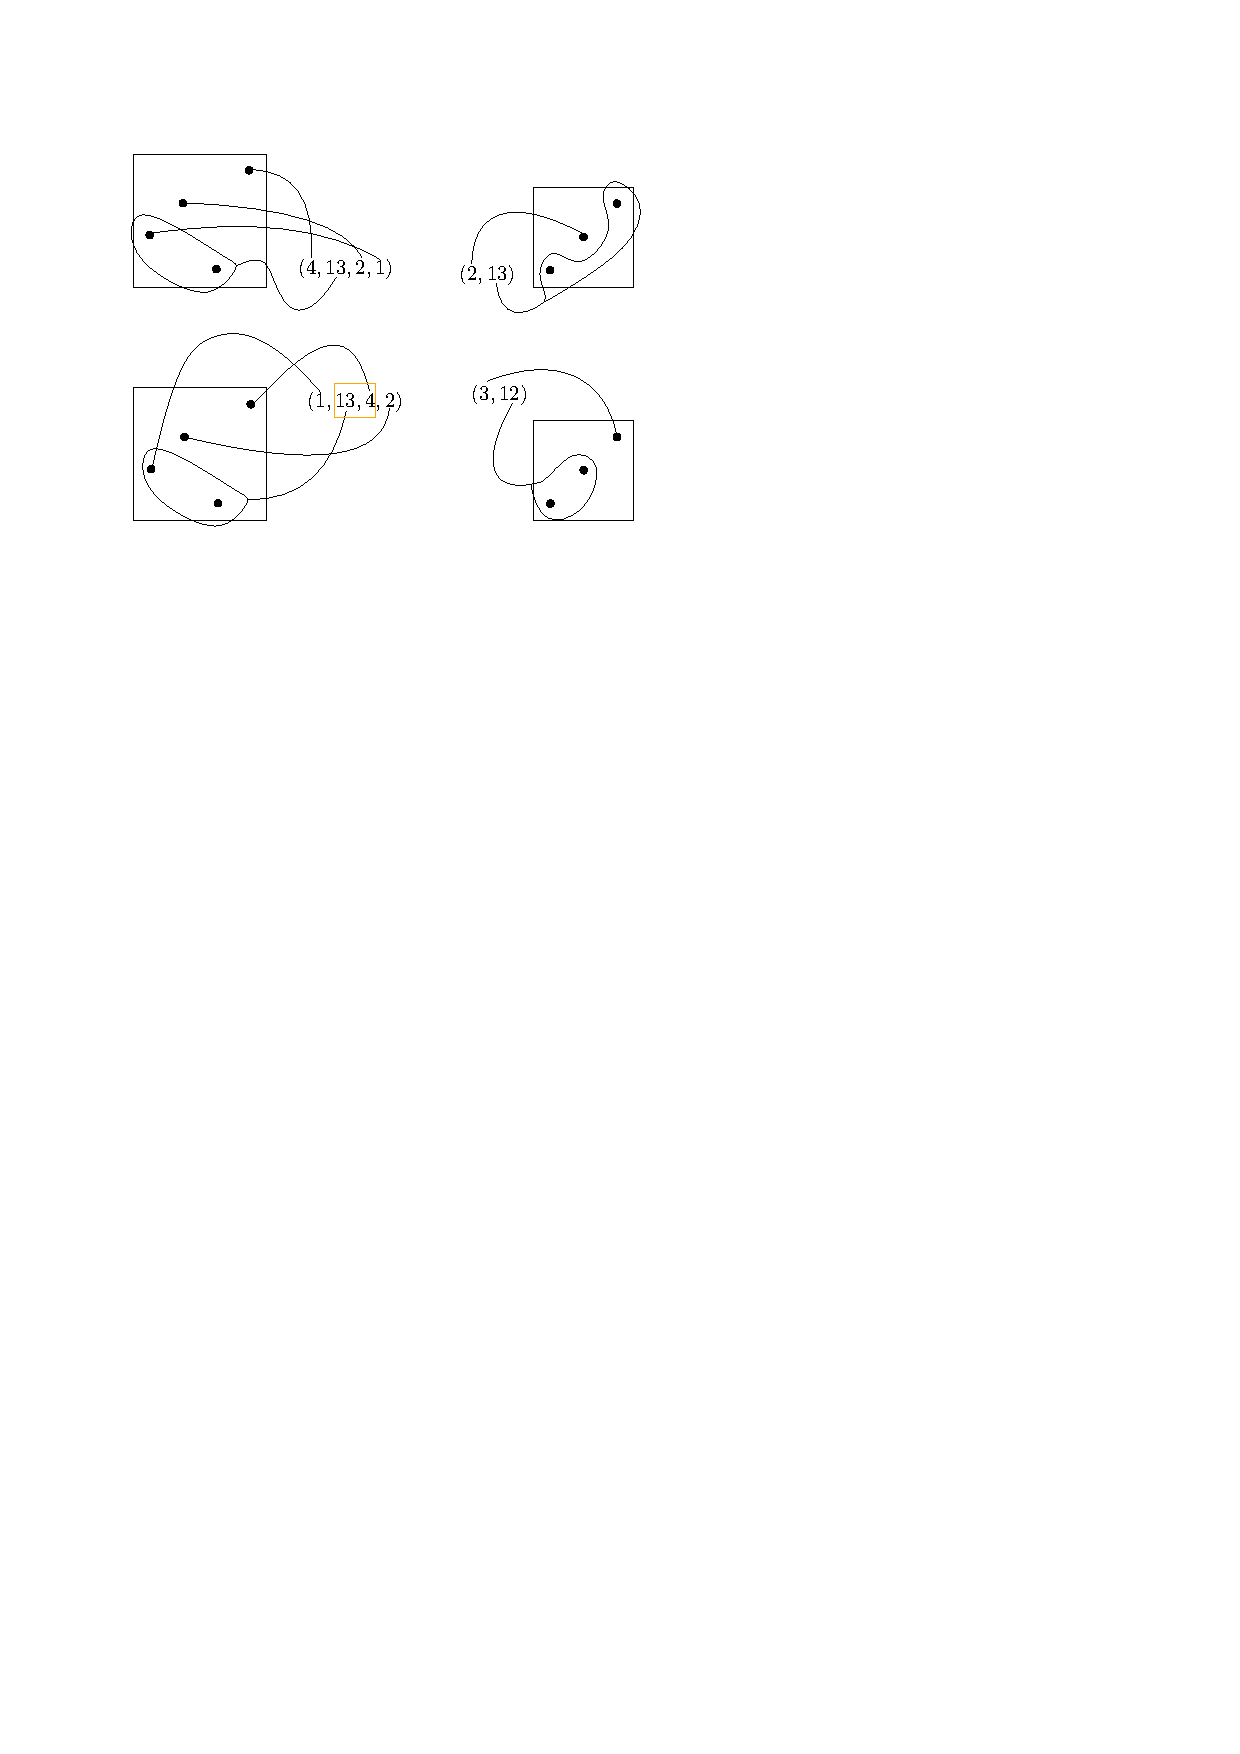
\includegraphics[scale=1]{../images/interlacing_25314.pdf}
    \caption{\textbf{From left to right:} the permutation 2314, along with a QSS from $1, 21, 1, 1$. Another QSS, this one is not interlacing: in orange the two sets that do not interlace. The permutation 123, along with its two interlacing QSS from $1, 12$.\label{fig:interlacingQSSsmpl}}
\end{figure}

\vspace{-.2in}

\begin{smpl}[Interlacing QSS]
The permutation $2314$ has several QSS from $1, 21, 1, 1$, for instance $(4, 13, 2, 1)$ and $(1, 13, 4, 2)$, but from these two, only the first is interlacing.
In \cref{fig:interlacingQSSsmpl}, one can see these two QSS.
Further computations can show that
\[\binom{2314}{1, 21, 1, 1} = 36 \quad \text{ and } \quad \begin{bmatrix}
2314 \\ 1, 21, 1, 1
\end{bmatrix} = 8.\]
One can observe that there are three QSS of $123$ from $1$, $12$, but one of them is non-interlacing (the QSS $(1,23)$), so
$\bigl[\!\begin{smallmatrix} 123 \\ 1, 21 \end{smallmatrix}\!\bigr] = 2$.
In \cref{fig:interlacingQSSsmpl}, one can see these two QSS.
\end{smpl}

\begin{thm}[Cancellation-free and groupping-free antipode formula for Permutation pattern Hopf algebra]\label{thm:antipode_perms_intro}
Let $\pi = \pi_1\oplus \dots \oplus \pi_n$ be the decomposition of a permutation $\pi$ into $\oplus$-indecomposable permutations.
Then, we have the following formula for the antipode of $\pat_{\pi}$:

$$S(\pat_{\pi}) = (-1)^n \sum_{\sigma} \begin{bmatrix}
\sigma \\ \pi_1, \dots, \pi_n
\end{bmatrix} \pat_{\sigma}\, ,$$
where the sum runs over all permutations $\sigma$, and the coefficients count the number of \textbf{interlacing QSS} of $\sigma$ from $\pi_1, \dots, \pi_n$.
\end{thm}
\begin{smpl}
Consider $\pi = 132 = 1 \oplus 21$.
It comes from the antipode axioms that the antipode on $\pat_{132}$ is:
$$S(\pat_{132}) =\pat_{132} + \pat_1 \pat_{21} = 3 \pat_{321} + 2 \pat_{231} + 2 \pat_{312} + \pat_{213} + 2 \pat_{21}\, . $$
%\begin{align*}
%S(\pat_{132}) =& \sum_{k=0}^2 (-1)^k \mu^{\circ k-1} \circ (\id_{\mathcal A(\mathtt{Per})} - \iota \circ \epsilon)^{\otimes k} \circ \Delta^{\circ k-1}(\pat_{132})\\
%=& - \underbrace{\pat_{132}}_{k=1} + \underbrace{\pat_1 \pat_{21}}_{k=2} 
%= 3 \pat_{321} + 2 \pat_{231} + 2 \pat_{312} + \pat_{213} + 2 \pat_{21} \, .
%\end{align*}
These coefficients can be seen as enumerating quasi-shuffle signatures of $132$ from $1$ and $12$ that are \textbf{interlacing}, according to \cref{thm:antipode_perms_intro}.
\end{smpl}
Similarly to the case of graphs, the antipode formula in \eqref{thm:antipode_perms_intro} begets reciprocity results, see \cref{sec:polynomial}. Also, the notion of \emph{bialgebra in cointeraction} (c.f. \cite{Foissy}) can also be used to obtain antipode formulas for the pattern Hopf algebra.
This is discussed in \cite{penaguiao2023polynomial}.

\section{The pattern Hopf algebra \label{sec:pattern_algebra_contruction}}

\begin{comment}
\subsection{Species}

Let $\mathbb{K}$ be a field of arbitrary characteristic. Let $\Fset$ be the category of finite sets and bijections between finite sets, and $\Vect_{\mathbb{K}}$ be the category of $\mathbb{K}$-vector spaces and linear maps between vector spaces. A {\bf vector species}, or simply a \textbf{species}, is a functor $\tp: \Fset \to \Vect_{\mathbb{K}}$. A morphism between species $\tp$ and $\tq$ is a natural transformation between the functors $\tp$ and $\tq$. We write $\Ss_{\mathbb{K}}$ for the category of vector species over the field $\mathbb{K}$. A {\bf monoid} (resp. {\bf comonoid}) in $\Ss_{\mathbb{K}}$ consists of a vector species $\tp$ equipped with a collection $\mu$ (resp. $\Delta$) of linear maps $\mu_{S,T}: \tp[S]\otimes \tp[T]\to \tp[I]$ (resp. $\Delta_{S,T}: \tp[I]\to \tp[S]\otimes \tp[T]$), subject to associativity and unitary axioms (resp. coassociativity and counitary axioms). A {\bf connected Hopf monoid} in $\Ss_{\mathbb{K}}$ is a vector species $\thh$ with $\thh[\emptyset]=\mathbb{K}$, endowed with a monoid and comonoid structure, subject to naturality and compatibility axioms.

We can also consider {\bf set species}, whose are simply functors $\rP: \Fset \to \Set$, where $\Set$ is the category of arbitrary sets and arbitrary maps between sets. It is possible to relate set species to vector species via the \emph{linearization functor} $\mathbb{K}(-): \Set \to \Vect_{\mathbb{K}}$, which sends a set to the vector space generated by the given set. Composing a set species $\rP$ with the linearization functor gives a vector species, denoted by $\mathbb{K}\rP$. A {\bf linearized species} is a vector species $\tp$ of the form $\tp=\mathbb{K}\rP$, for some set species $\rP$.

In general, the notions of monoid, comonoid, bimonoid and Hopf monoid for set species can be described in terms similar to those presented for vector species. The unique subtle difference is the comonoidal-structure analogue to set species: the only maps to the unit object are the ones obtained from species concentrated on the empty set. This implies that there are no nontrivial comonoids in the category of set species. Nevertheless, there exists a ``comonoid-like'' structure on set-species, introduced by Aguiar and Mahajan in \cite{AM2010}, for which the linearization of such comonoids results in a comonoid of vector species.

A {\bf comonoid in set species} consist of a species $\rP$ equipped with morphisms of species
\[\Delta:\rP \to \rP \cdot \rP \qquad \text{ and } \qquad \varepsilon: \rP \to \mathrm{1}_{\{\emptyset \} }. \]
That is, for each decomposition $I=S \sqcup T$ we have maps $\Delta_{S,T}: \rP[I]\to \rP[S] \times \rP[T]$, and $\varepsilon_\emptyset: \rP[\emptyset] \to \{\emptyset\}$. If $x \in \rP[I]$,  let 
\[(x|_S, x /_S)\in \rP[S]\times \rP[T]\]
denote the image of $(x,y)$ under $\Delta_{S,T}$. The map $x \mapsto x|_S$ can be thought as a ``restriction'' of the structure $x$ from $I$ to $S$, while $x \mapsto x/_S$ can be associated to a ``contraction'' of $S$ from $x$, resulting in a structure on $T$. The collection of maps $\Delta=(\Delta_{S,T})$, called the {\bf coproduct} of the set-species, must satisfy naturality, coassociativity and counit axioms analogues to the ones defined for monoids in vector species. 

In \cite{AM2010} (Part III), a construction is presented allowing to produce a (graded) Hopf algebra from a Hopf monoid.
We recall briefly this construction. Let $\mathbb{K}$ be a field of characteristic zero. If $\tp \in \Ssk$, then there is an action of the symmetric group $\mathfrak{S}_n$ on $\tp[n]$ by relabeling, for each $n \geq 0$. We denote by $\tp[n]_{\mathfrak{S}_n}$ the \emph{space of $\mathfrak{S}_n$-coinvariants of $\tp[n]$}:
\[
  \tp[n]_{\mathfrak{S}_n}:=\tp[n]/\left\langle \, x- \tp[\alpha](x) \, | \, \alpha \in \mathfrak{S}_n, x\in \tp[n] \,\right\rangle.
\]

Consider $\gVec$ be the category of graded vector spaces over $\mathbb{K}$. The functors $\Kc, \Kcb: \Ssk \to \gVec$ given by 
\[
    \Kc(\tp):=\bigoplus_{n \geq 0}\tp[n] \qquad , \qquad \Kcb(\tp):= \bigoplus_{n \geq 0}\tp[n]_{\mathfrak{S}_n}
\]
are referred in \cite{AM2010} as \emph{full Fock funtor} and \emph{bosonic Fock functor}, respectively. From any monoid (resp. comonoid, Hopf monoid) $\tp$, it is possible to obtain algebras (resp. coalgebras, Hopf algebras) $\Kc(\tp)$ and $\Kcb(\tp)$ from those of $\tp$, together with certain canonical transformations (see \cite{AM2010}, section 15.2).
\end{comment}

\subsection{Species with restriction}
The general setting for our approach to patterns is given by the notion of \emph{species with restrictions}, a terminology due to Schmitt (see \cite{Schmitt1993}) and used by the first author in\footnote{In this work, species with restrictions are called \emph{combinatorial presheaves}.} \cite{Penaguiao2020}.

Let $\mathbb{K}$ be a field of arbitrary characteristic. We denote by $\Fset$, $\Vect_{\mathbb{K}}$ and $\Fset_{\!\!\!\!\!\hookrightarrow}$ the category of finite sets and bijections between finite sets, the category of $\mathbb{K}$-vector spaces and linear maps between vector spaces and the category of finite sets with injections as morphisms, respectively. 
{\bf Set species}, {\bf vector species} and {\bf species with restriction} are defined respectively as contravariant functors $\rP: \Fset\to \Set$, $\tp:\Fset \to \Vect_{\mathbb{K}}$ and $\prR:\Fset_{\!\!\!\!\!\hookrightarrow} \to \Set$. Given a species with restrictions $\prR$ and two finite sets $I,J$ such that $J \subseteq I$, the {\bf restriction map} $\text{res}_{I,J}: \prR[I]\to \prR[J]$  is the image under the functor $\prR$ of the inclusion $J \hookrightarrow I$, so $\text{res}_{I,J}:=\prR[\hookrightarrow]$.
By functoriality, these maps satisfy the contravariant axioms
\begin{equation}\label{Axrestr}
    \text{res}_{J,K}\circ\text{res}_{I,J}=\text{res}_{I,K} \qquad , \qquad \text{res}_{I,I}=\text{id}_{\prR[I]},
\end{equation}
for any finite sets $I \supseteq J \supseteq K$. Set species, vector species and species with restrictions form  categories $\Ss$, $\Ss_{\mathbb{K}}$ and $\Spr$, respectively. In all those categories, the Cauchy product is denoted by $\cdot$.
This allows us to define \textbf{associative species with restrictions} in the usual way see \cite{Penaguiao2020}.

%Notice that, for any finite set $C$, the set species $\mathrm{1}_C$ is also a species with restrictions, where $\text{res}_{\emptyset, \emptyset} = \id_C$. 
Given a species with restrictions $\prR$, we can construct a linearized comonoid in $(\Ss, \cdot)$ as follows: Let $\trr=\mathbb{K}\prR$ be the linearization of $\prR$. Given a decomposition $I=S \sqcup T$, consider the linear map $\Delta_{S,T}: \trr[I]\to \trr[S] \otimes \trr[T]$ given by
\begin{equation}\label{CoprodRestr}
\Delta_{S,T}(x):=\text{res}_{I,S}(x)\otimes \text{res}_{I,T}(x),
\end{equation}
for any $x \in \prR[I]$. Let $\epsilon_\emptyset: \trr[\emptyset]\to \mathbb{K}$ the linear extension of the map sending every element of $\prR[\emptyset]$ to $1$. Hence, $(\trr, \Delta, \epsilon)$ is a linearized comonoid.


Consider now a linearized comonoid $\tp=\mathbb{K}\rP$ in $(\Ss, \cdot)$. 
That is a comonoid in set species that has no notion of restriction.
In this case, the coproduct gives a pure tensor
\[\Delta_{S.T}(x)=x|_S \otimes x/_S,\]
for each $x \in \rP[I]$ and for each decomposition $I = S \sqcup T$. We may then define restriction maps on $\tp$ either by the rule $x\mapsto x|_J$ or $x\mapsto x/_{I\setminus J}$ for $x \in \tp[I]$. Each of this two restriction maps turns $\tp$ into a species with restriction. When $\tp$ is cocommutative, then both restriction maps coincide. We have then the following characterization of monoids of species with restrictions (see \cite{AM2010}, Proposition 8.29, for other characterizations).

\begin{thm}[Schmitt, Aguiar-Mahajan]\label{thm:swr_lcc}
There is an equivalence between the category of monoids in $(\Spr, \cdot)$ and the category of linearized cocommutative bimonoids.
\end{thm}

\subsection{Pattern functions and the pattern Hopf algebra}

Given a species with restrictions $\prR$ and two finite sets $I$ and $J$, two objects $a\in \prR[I], b\in \prR[J]$ are said to be {\bf isomorphic objects}, or $a\sim b$, if there is a bijection $\sigma:I\to J$ such that $\prR[\sigma](b)=a$. The collection of equivalence classes of a species with restrictions $\prR$ is denoted by $\mathcal{G}(\prR) := \bigcup_{n\geq 0 } \prR[n]_{\mathfrak{S}_n}$. 
In this way, the set $\mathcal G(\prR) $ is the collection of all the $\prR$-objects up to isomorphism. 
%It is straightforward to show that $\mathcal{G}(\prR)$ is a basis for the vector space $\Kcb(\prR)$. 
Recall that for every two finite set $I,J$ such that $J \subseteq I$, there is a restriction map $\text{res}_{I,J}: \prR[I] \to \prR[J]$, defined as the image by $\prR$ of the map $J \hookrightarrow I$. If $b \in \prR[I]$, we write $b|_J \coloneqq\text{res}_{I,J}(b)$.

\begin{defin}[Patterns coefficients]\label{defin:patterncoeff}
Let $\prR$ be a species with restrictions. Given two finite sets $I,J$ such that $J \subseteq I$ and two objects $b\in \prR[I], a\in \prR[K]$,
we say that the subset $J \subseteq I$ is a {\bf pattern} of $a$ in $b$ if $b|_J \sim a$. More precisely, $J \subseteq I$ is a pattern of $a$ in $b$ if there exists a bijection $\sigma: J \to K$ such that $\prR[\sigma](a)=\text{res}_{I,J}(b)$. The {\bf pattern coefficient} of $a$ in $b$ is
\begin{equation}
    \binom{b}{a}_{\!\prR} \coloneqq \pat_a(b) \coloneqq \left| \{J \subseteq I \, : \, b|_J \sim a \} \right| \, .
\end{equation}
\end{defin}

From \cite{Penaguiao2020}, this number only depends on the isomorphism classes of $a \in \prR[J]$ and $b \in \prR[I]$.
%This motivates the following notion.

\begin{defin}[Patterns functions and patterns spaces]\label{defin:pattern}
Let $\prR$ be a species with restrictions. Given a finite set $I$, we define the {\bf pattern function} associated to $a \in \prR[I]$ as the function $\pat_a: \mathcal{G}(\prR) \to \mathbb{K}$
given by $\displaystyle b \mapsto \pat_a(b)$\, ,
for all $b \in \mathcal{G}(\prR)$. The linear span of the pattern functions is denoted by $\mathcal{A}(\prR):=\mathbb{K}\{\pat_a \, : \, a\in \mathcal{G}(\prR)\}$.
\end{defin}

\begin{comment}
By definition $\pat_a \in \mathcal{F}(\mathcal{G}(\prR), \mathbb{K})$, where $\mathcal{F}(\mathcal{G}(\prR), \mathbb{K})$ denotes the set of functions from $\mathcal{G}(\prR)$ to $\mathbb{K}$. Without loss of generality, we denotes by $\pat_a$ the linear extension of the pattern function associated to $a$. Hence, we can consider $\{ \pat_a \}_{a\in \mathcal{G}(\prR)}$ as a family of linear functions from $\Kcb(\prR)$ to $\mathbb{K}$, indexed by $\mathcal{G}(\prR)$.
In \cref{sec:speciespermutation}, we see an example of a species with restrictions structure on permutations.
\end{comment}

\begin{comment}
\begin{defin}[Patterns space]
If $\prR$ is a species with restriction, then the linear span of the pattern functions is denoted by
\begin{equation}
    \mathcal{A}(\prR):=\mathbb{K}\{\pat_a \, : \, a\in \mathcal{G}(\prR)\}.
\end{equation}
\end{defin}
\end{comment}


\begin{thm}[\cite{Penaguiao2020}]
Let $(\prR, \sq, 1) $ be an associative species with restrictions. The space $\mathcal{A}(\prR)$ is closed under pointwise multiplication and has a unit.
It forms an algebra, called the {\bf pattern algebra associated to} $\prR$.
More precisely, if $a, b \in \mathcal G(\prR)$,
\begin{equation}\label{eq:prodrule}
\pat_ a   \pat_b = \sum_c \binom{c}{a, b}_{\! \prR} \pat_c \, ,
\end{equation}
where the coefficients $\binom{c}{a, b}_{\!\prR}$ are the number of ``quasi-shuffles'' of $a, b$ that result in $c$, specifically, if we take $c\in \prR[C]$ to be a representative of the equivalence class $c$, then:
$$ \binom{c}{a, b}_{\!\prR} = \left| \{(I, J) \, \text{ such that } \, \,  I \cup J = C \, ,\, \, c|_{I} \sim a, \, c|_{J} \sim b \} \right| \, .  $$

If we also consider the following coproduct in the pattern algebra $\mathcal A (\prR)$:
\begin{equation}\label{eq:coprodformula}
\Delta_{\sq} \pat_ a = \sum_{\substack{ b, c \, \in \, \mathcal G (\prR) \\ a = b \, \sq \, c}} \pat_b \otimes \pat_c \, ,
\end{equation}
then the pattern algebra of $\prR$ together with the coproduct $\Delta_{\sq}$, and a natural choice of counit, forms a bialgebra.
If additionally $| \prR[\emptyset ] | = 1 $, it forms a filtered Hopf algebra.
\end{thm} 


%\section{Examples of species with restrictions \label{sec:species_restrictions}}

%\subsection{Species on linear orders.\label{sec:specieslinearorders}}

%The set species of total orders $\mathtt{L}$ is defined has $\mathtt{L}[I] = \{\text{ total orders in $I$ }\}$.
%The restriction of an order $\leq \in \mathtt{L}[I]$ to a subset $J$ is the induced order, which is a total order.
%This defines a species with restrictions, which is also a monoid with the concatenation product $*$. 

%If $\mathsf{p} \in \mathtt{L}[I]$, we write $\mathbb{X}(\mathsf{p}) = I$. It is straightforward to show that, for every species with restriction $\mathsf{r}$, then $I$ is an order ideal in $\mathsf{p} \ast \mathsf{r}$ if $\mathbb{X}(\mathsf{p}) = I$ (see \cite{PV2022}, Proposition 5.1).


\begin{comment}
We also define an associative structure on $\mathtt{L}$.
If $\mathsf{p}$ is a total order in $I$ and $\mathsf{r}$ is a total order in $J$, and if $I, J$ are disjoint, then we can define $\mathsf{p} \ast\mathsf{r}$ a total order on $I \sqcup J$ as:
\begin{itemize}
\item if $a, b \in I$ such that $a \, \mathsf{p} \, b$, then $a \, \mathsf{p} \ast \mathsf{r} \, b$.

\item if $a, b \in J$ such that $a \, \mathsf{r} \, b$, then $a \, \mathsf{p} \ast \mathsf{r} \, b$.

\item if $a \in I$ and $b \in J$, then $a \, \mathsf{p} \ast \mathsf{r} \, b$.
\end{itemize}
This is invariant up to restrictions and relabellings, so this builds a connected associative species with restrictions. 


If $\mathsf{p} \in \mathtt{L}[I]$, we write $\mathbb{X}(\mathsf{p}) = I$.
The following fact is an immediate observation.

\begin{prop}\label{prop:linorderideals}
If $\mathbb{X}(\mathsf{p}) = I$, then $I$ is an order ideal in $\mathsf{p} \ast \mathsf{r}$.
\end{prop}
\end{comment}


\subsection{Species on linear orders, permutations and packed words\label{sec:speciespermutation}}

The set species of linear orders, $\mathtt{L}$ is defined has $\mathtt{L}[I] = \{\text{ total orders in $I$ }\}$.
This can be endowed with a notion of restriction and product quite canonically.

We will generalize the framework used in \cite{albert2020two}, where a rather unusual definition of permutations was introduced, in order to defines our species with restriction on permutations and packed words.  
First, we call a linear partial order $\leq$ on a set $I$ the pullback of a surjective map $I \to [m]$.
We call this function the rank of $\leq$, or $rk_{\leq}$.
We abuse notation and also call the integer $m$ the rank of the order $\leq$.

\begin{figure}[h]
	\centering
	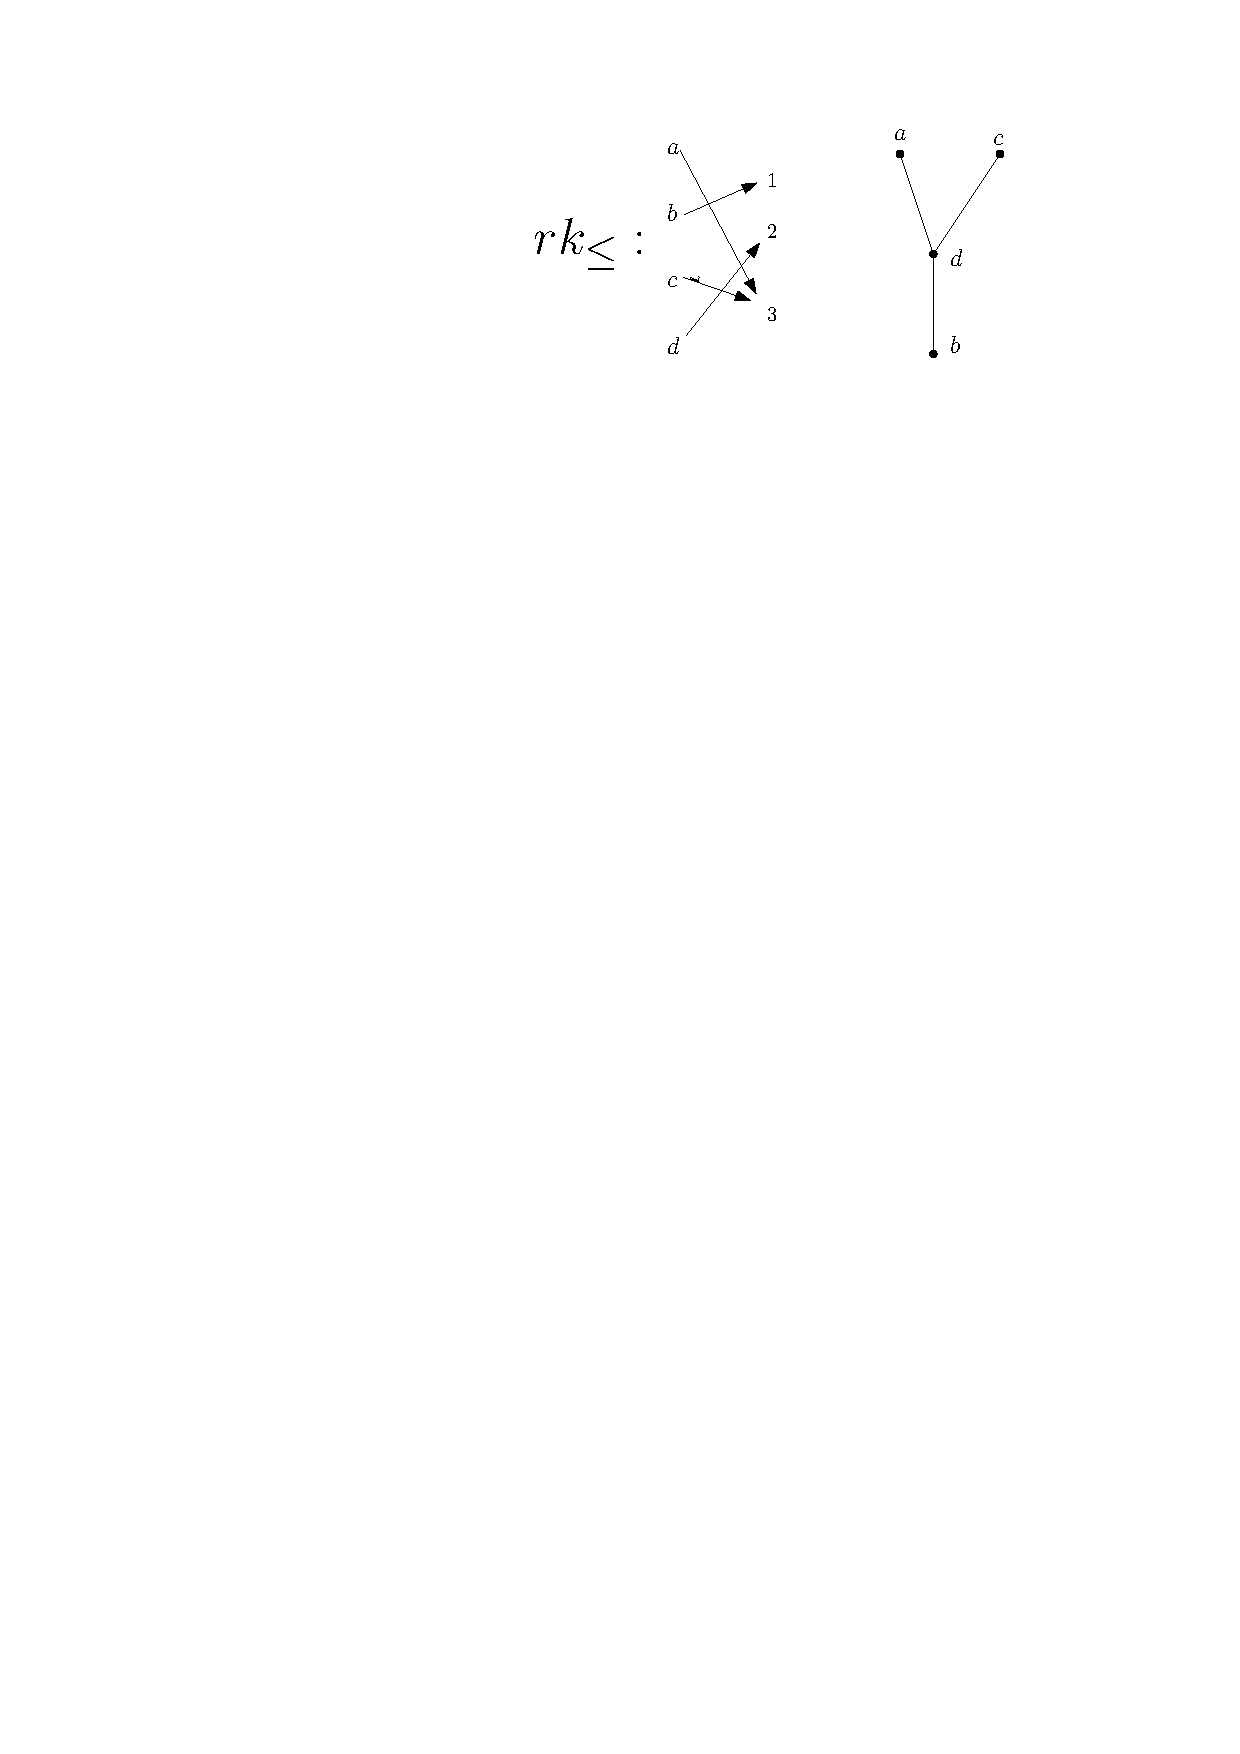
\includegraphics[scale=.9]{../images/packedWordOrder.pdf}
	\caption{\textbf{Left:} If $f = \{ a\mapsto 3, b\mapsto 1, c\mapsto 3, d\mapsto 2\}$ is a surjective map $\{a, b, c, d\}\to[3]$, the inherited order is $\{b < d < \{a, c \}\}$ and has rank three. \textbf{Right:} The Hasse diagram of the linear partial order inherited by $f$. \label{fig:packedWordOrder}}
\end{figure}

In this way, a permutation $\pi$ on $I$ is a pair of total orders ($\leq_P, \leq_V)$, and a packed word $\omega$ on $I$ is a pair of orders $(\leq_P, \leq_V)$ where $\leq_P$ is a total order in $I$, and $\leq_V$ is a linear partial order on $I$.
In particular, note that any permutation on $I$ can be seen as a packed word on $I$, as any total order is a linear partial order.
This relates to the usual notion of packed words as a word in $[m]$ in the following way:
if we order the elements of $I = \{a_1 \leq_P \dots \leq_P a_k \}$, then the corresponding packed word is $rk_{\leq_V}(a_1)rk_{\leq_V}(a_2) \dots rk_{\leq_V}(a_k) \, $. Conversely, for any packed word $\omega = p_1\dots p_k$, there are several pairs of isomorphic orders $(\leq_P, \leq_V)$ corresponding to the word $\omega$. If $I \hookrightarrow J$, by restricting the orders on $I$ to orders on $J$, we obtain a restriction to a packed word on $J$, which results on species with restrictions structures denoted by $\mathtt{Per}$ and $\mathtt{PWo}$.

It will be useful to represent packed words $\omega $ in $I$ as rectangle diagrams labeled by $I$.
This is done in the following way: let $1\leq m \leq |I|$ be the rank of $\omega$, we place the elements of $I$ in an $m \times |I|$ grid so that the elements are placed horizontally according to the $\leq_P$ order, and vertically according to the $\leq_V$ order.
\begin{figure}[h]
\[\footnotesize{
\begin{array}{|c|c|c|}
	\hline & & 3 \\
    \hline 1 & &  \\
    \hline & 2 & \\
    \hline 
\end{array} \qquad , \qquad 
\begin{array}{|c|c|c|c|c|}
	\hline   & e &   &   & b \\
    \hline   &   &   & a &   \\
    \hline d &   & c &   &   \\
    \hline 
\end{array}}\, \, \, .\]
\caption{{\bf Left}: permutation $\pi = \{1<_P2<_P3 , 2<_V1<_V3\}$ in $\{1, 2, 3\}$. {\bf Right}: packed word $\omega = 13123 = \{ d > e > c > a > b, \{b, e\} > \{a\} > \{d, c\}\}$ in $\{a, b, c, d, e\}$.}
\end{figure}


If $f:J \to I $ is an injective map, the preimage of each order $\leq_P, \leq_V$ is well defined.
Furthermore, the preimage of $\leq_P$ is a total order on $J$, whereas the preimage of $\leq_V$ is a total order on $J$.
Thus, this defines the packed word $\mathtt{PWo}[f](\omega )$.
The $\ast $ operation on partial orders can be extended to a \textbf{diagonal sum} operation $\oplus $ on packed words.
This is the shifted concatenation of packed words.
This endows both $\mathtt{Per}$ and $\mathtt{PWo}$ with an associative species with restrictions structure.

\subsection{Species on parking functions}

A {\bf parking function} $\mathfrak{p} = a_1 \dots a_n$ is a sequence of integers in $[n]$ such that, after reordering $a^{(1)} \leq a^{(2)} \leq \dots \leq a^{(n)}$, we have $a^{(i)} \leq i$ for all $i$. Given an $n\times n$ square grid, a \textbf{Dyck path} on this square is an edge path, from the lower left corner to the upper right corner, that is always above the main diagonal.
It is a classical result that the number of Dyck paths of size $n$ is enumerated by Catalan numbers.

In \cite{PV2022} we describe a structure of species with restrictions on parking functions $\mathtt{PF}$, by leveraging a recent construction of parking functions via labelled Dyck paths, see \cite{BGLPV2021}.
%The species of \textbf{parking functions} $\mathtt{PF}$ is defined by letting $\mathtt{PF}[I]$ be the collection of all parking functions $\mathfrak{p} = \mathfrak{p}(I, \mathcal D, f, \leq)$, that is Dyck paths $\mathcal D$ in an $|I|\times |I|$ grid, labelled by elements of $I$ along with an order $\leq$ of $I$.
%We can give it a notion of species with restrictions: for each inclusion $\iota : I \hookrightarrow J $ and a labelled Dyck path $(J, \mathcal D, f, \leq)$ on $J$, the restriction $\mathtt{PF}[\iota](J, \mathcal D, f, \leq) = (I, \mathcal D|_I, f|_I, \leq|_I)$ has an intuitive meaning, except perhaps for
%$\mathcal D|_I$, which we clarify in the following.
This is done via a notion of \textbf{tunnels}, introduced by Deutsch and Elizalde in \cite{elizalde2003simple}, and is described in \cref{fig:restriction_parking}.
In particular, it recovers a notion of patterns in parking functions studied in \cite{adeniran2022pattern}. 
One further defines a shifted concatenation $\oplus$ on parking functions.




\begin{figure}[h]
\centering
    \subfloat[\centering The parking function 31411 and its restriction]{{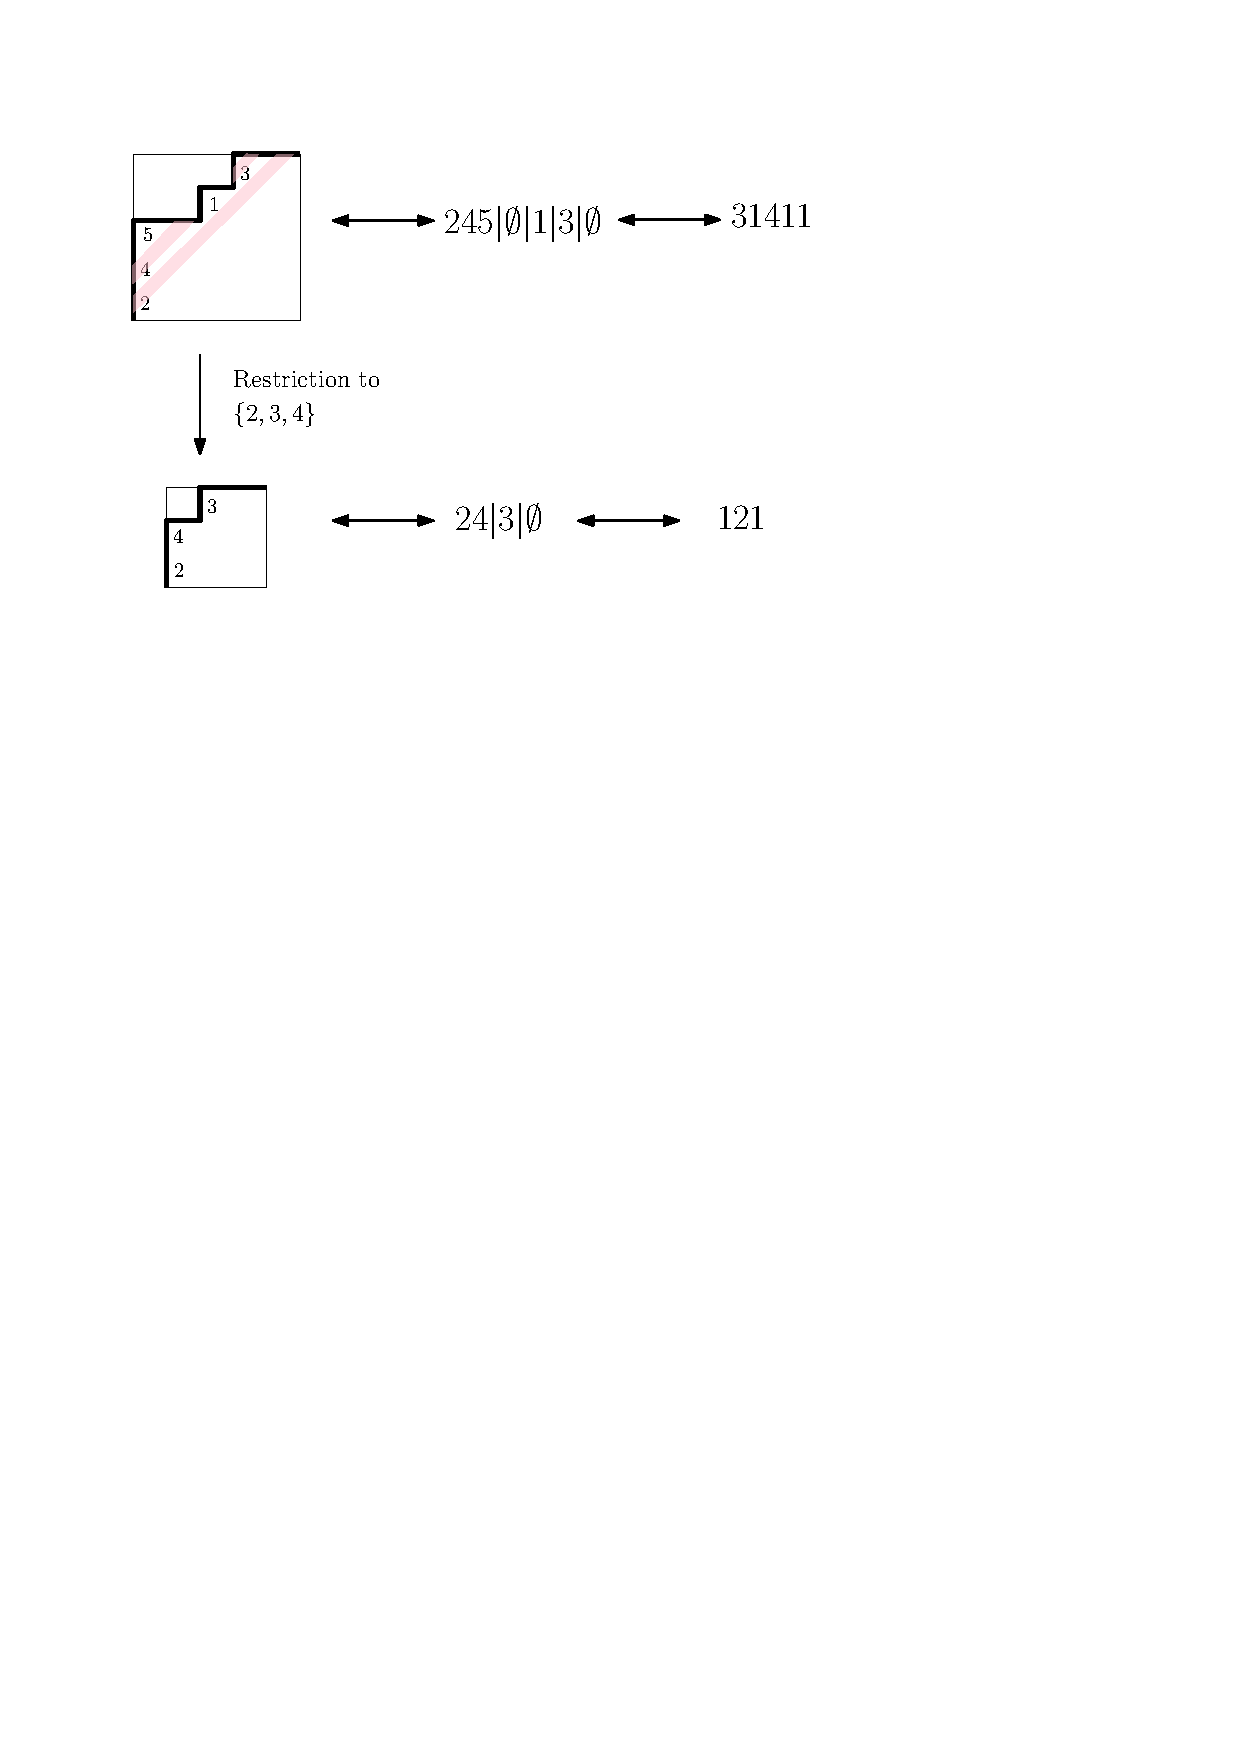
\includegraphics[height=4.9cm]{../images/restrictions_parking.pdf} }}%
    \qquad
    \subfloat[\centering The parking function 41511 and its restriction]{{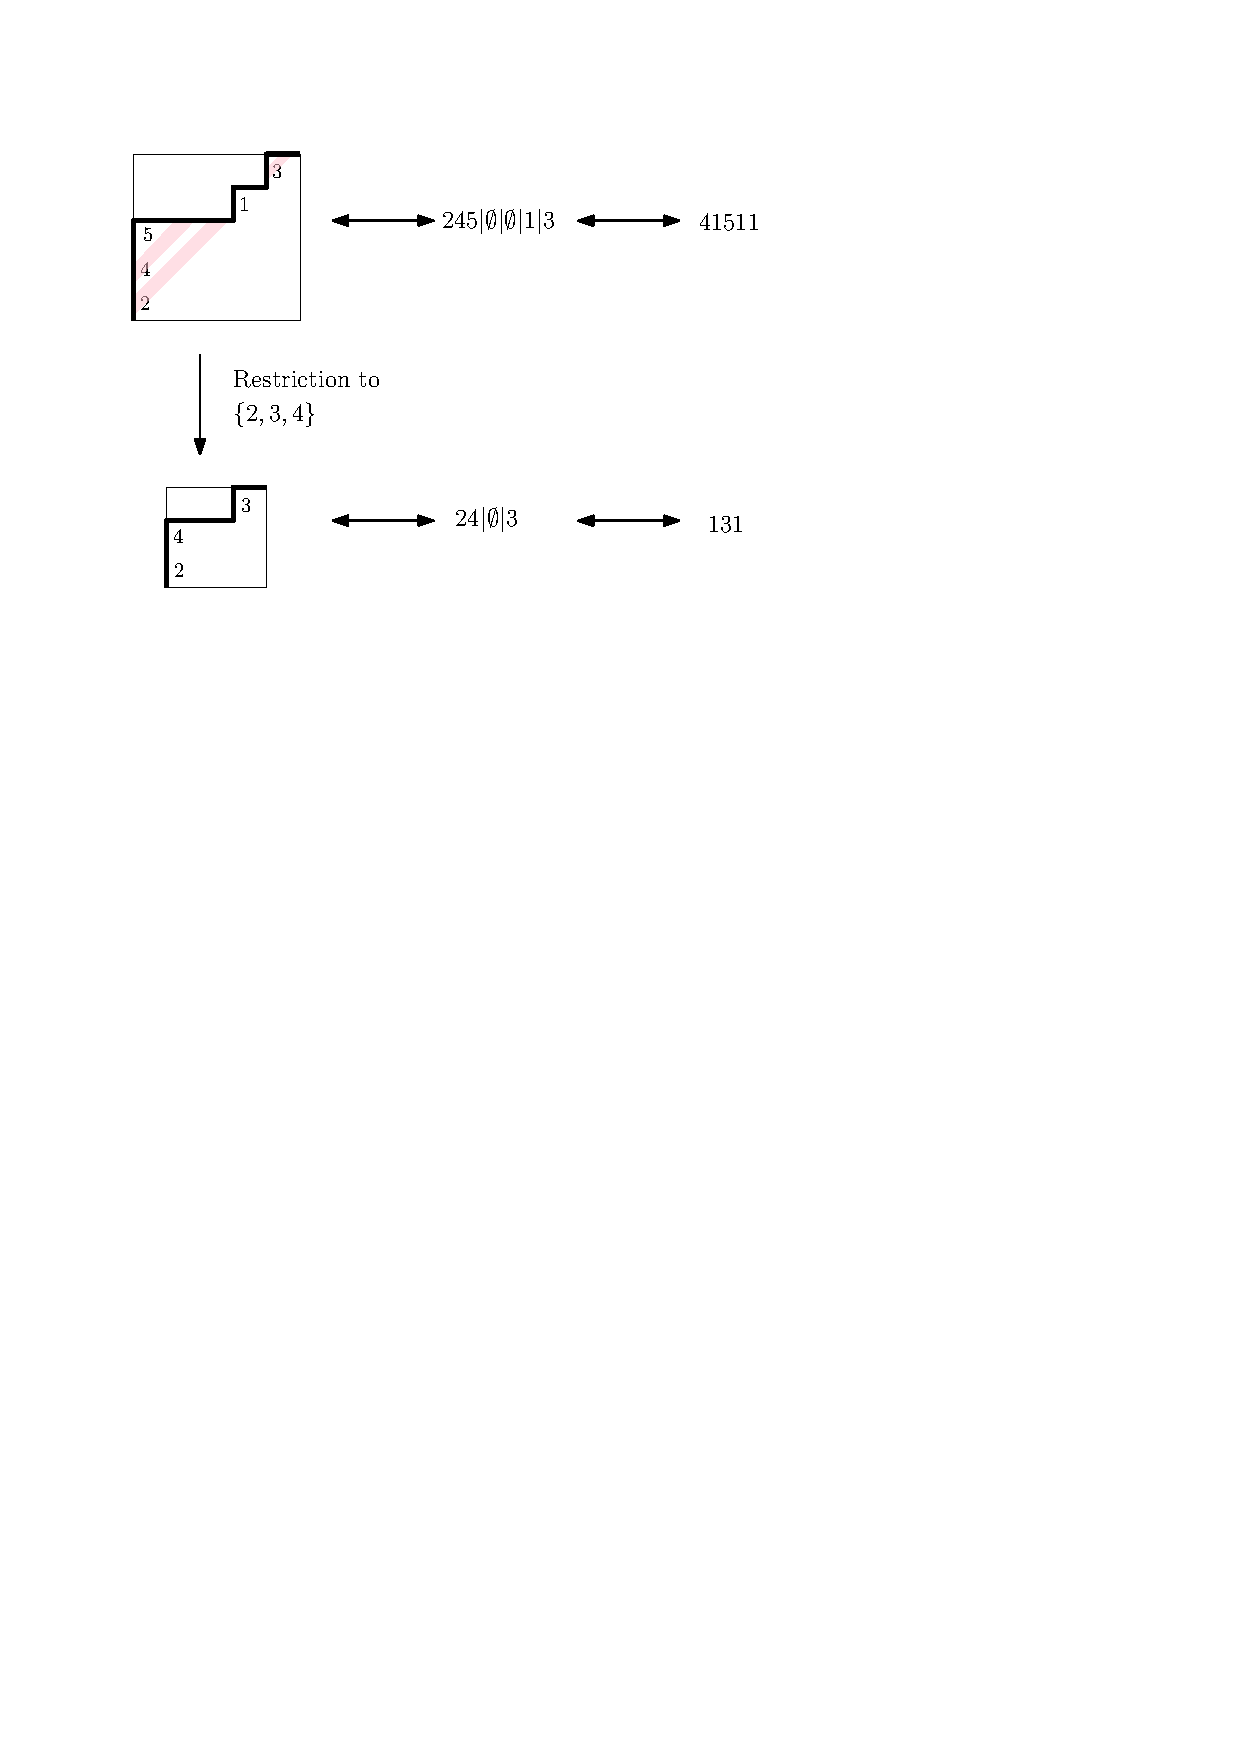
\includegraphics[height=4.9cm]{../images/restrictions_parking_other.pdf}}}%
    \caption{\label{fig:restriction_parking}}%
\end{figure}

The following can be established by the same methods presented in \cite{Penaguiao2020}.

\begin{prop}[Species with restrictions on parking functions]
The species $\mathtt{PF}$ forms a species with restrictions structure.
Furthermore,  $\oplus $ endows $\mathtt{PF}$ with a monoid structure, and the resulting Hopf algebra $\mathcal A(\mathtt{PF})$ is NCF, therefore it is free (see \cref{lm:freeness}).
\end{prop}


\section{$\mathtt{L}\times -$ species with restrictions}

In \cite[Corollary 3.4.]{Penaguiao2020} it was shown that in species with restrictions $\mathtt{h}$, any factorization into $\ast$-indecomposibles is unique up to order.
In some species with restrictions, we can also drop the ``up to order'' adjective, as there is exactly one factorization into $\ast$-indecomposibles full stop. We precise this in the \textit{non-commuting factorization} definition.
%We will be using $\star$ for the operation on $\End (H)$ and we will be using $\ast $ for the associative structure on a species.

\begin{defin}[Non-Commuting Factorization on pattern Hopf algebras]\label{defin:ncf}
A monoidal species with restrictions is called a \textbf{non-commuting factorization} species, or simply an NCF species, if any element $x$ has a unique factorization into $\ast$-indecomposibles elements $x = x_1 \ast \dots \ast x_n$.
\end{defin}

\begin{lm}[Linear species with restrictions have NCF, \cite{PV2022}, Lemma 6.2]\label{lm:freeness}
Let $\mathtt{R}$ be a connected species with restrictions.
Then $\mathtt{L} \times \mathtt{R}$ has NCF. Furthermore, $\mathcal A(\mathtt{R})$ is free.
\end{lm}

The last part of the above lemma is deduced from \cite{Vargas}, after we recognize that $\mathtt{L} \times \mathtt{R}'$ has NCF. In the following, we will refer to associative and connected species of the form $\mathtt{L} \times \mathtt{R}$ as \textbf{ordered species with restrictions}. The pattern Hopf algebra on permutations, on packed words and on parking functions all satisfy the NCF property.
In fact, permutations, packed words and parking functions are of the form $\mathtt{L} \times \mathtt{R}$.
This property allows for an easy manipulation of the coproduct, and results in a more tractable approach to the antipode formula.

\begin{defin}[Composition poset and cumulative sum]
Recall that we write $\mathcal C_n$ for the set of compositions of size $n$.
We will define the bijection $\mathbf{CS}:\mathcal C_n \to 2^{[n-1]}$, as follows.
If $\alpha =(\alpha_1, \dots, \alpha_{\ell} ) \in \mathcal C_n$, define $f_i = \sum_{j=1}^i \alpha_j$ and $\mathbf{CS}(\alpha) \coloneqq \{f_i\, | \, i = 1, \dots, \ell - 1\} \, $.


This bijection allows us to define an order $\leq $ in $\mathcal C_n$, via the pullback from the boolean poset in $2^{[n-1]}$.
This order can be defined as well as follows: we say that $\alpha \leq \beta$ if $\alpha$ arises from $\beta $ after merging and adding consecutive entries.
\end{defin}

\begin{comment}
Recall that a QSS $\III = (I_1, \dots , I_n)$ of $y\in \mathtt{R}[I]$ from $x_1, \dots, x_n$ satisfies $y|_{I_i} = x_i$ for all $i = 1, \dots , n$, and $I = \bigcup_i I_i$.
\end{comment}

\begin{defin}[Compositions and QSS]
Consider again $\mathtt{R}$ an ordered species with restrictions.
Let $x \in \mathtt{R}[J], y \in  \mathtt{R}[I]$, and $x = x_1\ast \dots \ast x_n$ be the unique factorization of $x$ into indecomposables.
Further say that $y = (\leq_y, \iota)$, where $\leq_y$ is a total order in $I$.
Let $\III = (I_1, \dots , I_n)$ be a QSS of $y$ from $x_1, \dots, x_n$ and consider a composition $\alpha \models n$.


Suppose that $ \mathbf{CS} (\alpha) = \{f_1, \dots, f_{\ell(\alpha) - 1} \}$ and use the convention that $f_0 = 0$ and $f_{\ell(\alpha)} = n$. 
Then we define for $i = 1, \dots, \ell(\alpha)$:
\[I^{\alpha}_i := I_{f_{i-1} + 1} \cup \dots \cup I_{f_i} \quad , \quad x^{\alpha}_i := x_{f_{i-1} + 1} \ast \dots \ast x_{f_i}.\]


For a partial order $\leq$ on a set $I$, and two sets $A, B \subseteq I$, we say that $A \lneq B$ if $A, B$ are disjoint and $a \leq b$ for any $a \in A$ and $b \in B$. Two indices $i< j$ are said to be \textbf{merged} by $\alpha$ if there is some $k$ in $\{1, \dots, n\}$ such that $ f_{k-1} < i < j \leq f_k$.
We say that a QSS $\III$ of $y$ from $x_1, \dots , x_n$ is $\alpha $-stable if $(I^{\alpha}_i)_i \text{ is a QSS of $y$ from } (x^{\alpha}_i)_i$ and, whenever $x_i \sim x_j$ and $i < j$ are merged with $\alpha $, then $I_i \lneq_y I_j$. Finally, we define 
\begin{equation}
   \mathcal I^{x, y}_{\III} \coloneqq \left\{ \alpha \models n \,\Big| \,\III \text{ is an $\alpha$-stable QSS of $y$ from } (x_i)_i \right\} \, . 
\end{equation}
\end{defin}

\begin{smpl}[$\alpha$-stable QSS on $\mathtt{PWo}$]
Consider the packed word $\rho = 21 \oplus 111 = 21333 = (1 < 2 < 3 < 4 < 5, 2 < 1 < \{3, 4, 5\})$ on the set $[5]$.
This packed word has three QSS from $21, 1, 11$, precisely $\III_1 =(12, 3, 45)$, $\III_2 =(12, 4, 35)$ and $\III_3 =(12, 5, 34)$.
All three are $(1, 1, 1)$-stable. We now observe that $\III_1, \III_2$ and $\III_3$ are $(2, 1)$-stable, but neither $(1, 2)$-stable nor $(3)$-stable.
Indeed, $\III_1^{(1, 2)} = \III_2^{(1, 2)} = \III_3^{(1, 2)} = (12, 345)$, and $\rho|_{345} = 111$ is not $\rho|_{I_2} \oplus \rho|_{I_3}$ for any of the QSS.
On the other hand, $\III_1^{(2, 1)} = (123, 45)$, $\III_2^{(2, 1)} = (124, 35)$ and $\III_3^{(2, 1)} = (125, 34)$, in each case is easy to note that $\rho|_{I_1^{(2, 1)}} = 21\oplus 1$ and $\rho|_{I_2^{(2, 1)}} = 11$ for each of the QSS. Therefore, in each case we get
$\mathcal I_{\III}^{21\oplus 1\oplus 11, 21333} = \{(1, 1, 1), (2, 1)\}\, $.
\end{smpl}
Define the composition $\mu_i \coloneqq (\underbrace{1, \dots , 1}_\text{$i-1$ times}, 2, 1, \dots, 1)$.
If $\III = (I_1, \dots, I_n)$  is a $\mu_i$-stable QSS, then $y|_{I_1 \cup I_{i+1}} = y|_{I_i} \ast y|_{I_{i+1}}$.
This motivates the following lemma.

\begin{lm}[\cite{PV2022}, Lemma 6.2]\label{obs:pwords-characterisation}
Let $\mathtt{R}$ be an ordered species with restriction.
Consider $x, y$ objects in $\mathtt{R}$, such that $y = (\leq_y, m)$ and $x = x_1\ast \dots \ast x_n$ a factorization into indecomposibles.
If $\III = (I_1, \dots, I_n)$ is a QSS of $y$ from $x_1, \dots x_n$ that is $\mu_i$-stable, then $I_i \lneq_y I_{i+1}$.
\end{lm}

In the case of packed words, a stronger claim can be used to compute $\alpha$-stability (see \cref{lm:QSSpackedWords}). Also, if $\mathtt{R}$ is a species with restrictions, $y, x_1, \dots, x_n \in \mathcal G(\mathtt{R})$ and $\III$ a QSS of $y$ from $x_1\dots, x_n$, then $\mathcal I^{x_1 \ast \dots \ast x_n, y}_{\III}$ has a unique maximal element, $\mathbb{1} = (1, \dots, 1)$.

\begin{thm}[\cite{PV2022}, Theorem 6.10]\label{thm:general_antipode}
For an ordered species with restrictions $\mathtt{R}$, and an element $x$, along with its factorization $x=x_1 \ast \dots \ast x_n$, the antipode of $\mathcal A (\mathtt{R})$ is given by:

$$S(\pat_x) = \sum_y \pat_y \sum_{\substack{\III \text{ QSS of $y$}\\ \text{from }x_1, \dots , x_n}}  \sum_{\alpha \in \mathcal I^{x, y}_{\III}} (-1)^{\ell ( \alpha)} \, .$$
\end{thm}

%\begin{smpl}[Example in permutation patterns]
%Consider $\sigma = 312$ and $\pi = 123 = 1\oplus 1 \oplus 1$.
%We will compute the antipode of $\pat_{\sigma}$ using this formula, by computing $\mathcal I^{\sigma, \pi}_{\III}$ for each QSS $\III$.
%
%\end{smpl}

\begin{prop}[Filtered structure of $\mathcal I$, \cite{PV2022}, Proposition 6.11] \label{prop:filter_structure_I}
For an ordered species with restrictions $\mathtt{R}$, and an elements $x\in  \mathtt{R}[J], y\in \mathtt{R}[I]$, along with a factorization into $\ast$-indecomposibles $x = x_1 \ast \dots \ast x_n$ and a QSS $\III$ of $y$ from $x_1, \dots, x_n$, we have that $\mathcal I^{ x, y}_{\III}$ is a filter.
That is, if $\alpha \in \mathcal I^{ x, y}_{\III}$ and $\beta \geq \alpha$ then $\beta \in \mathcal I^{ x, y}_{\III}$. Furthermore, if $\mathcal I^{ x, y}_{\III}$ has a unique minimal element distinct from $\mathbb{1}$, then $\sum_{\alpha \in \mathcal I^{x, y}_{\III}} (-1)^{\ell(\alpha)} = 0 \, $.
\end{prop}


%We use the bijection $\mathbf{CS}$ between compositions and subsets of $\{1, \dots , n-1\}$ to compute the following sum.
%Let $X \coloneqq \mathbf{CS}(\mathbb{0} )$, then we can consider $\zeta : \mathcal K \to \mathcal K$

%\begin{align*}
%\sum_{\alpha \in \mathcal I^{y, x}_{\III}} (-1)^{\ell(\alpha)} &= \sum_{X \subseteq Y \subseteq [n-1]} (-1)^{|Y| +1} = \sum_{k = |X|}^{n-1} \sum_{\substack{X \subseteq Y \subseteq [n-1]\\ |Y| = k}} (-1)^{k +1} \\
%&= \sum_{k = |X|}^{n-1}\binom{n-|X| - 1}{k - |X|} (-1)^{k +1} = \sum_{k = 0}^{n- |X|-1}\binom{n-|X| - 1}{k} (-1)^{k + |X| +1}  \\
%&= (1 -1)^{n - |X| - 1 + |X| +1} = 0 \, .\\
%\end{align*}

%Notice that because $X \neq [n-1]$, we can use the Newton identity with exponent $n-|X| - 1$.

The consequence is, for pattern algebras, that computing the antipode corresponds to find which $\mathcal I_{\III}^{x, y}$ have a unique minimal element.
In this case, the antipode formula reduces to counting how many of these minimal elements are the composition $\mathbb{1}$.
These will contribute with $(-1)^n$ to the total coefficient of $\pat_y$.

%\section{The antipode formula on special cases\label{sec:formula_pp}}
\section{The antipode formula for the pattern algebra on packed words\label{sec:formula_packed}}
%Let $\rho = (\leq_P, \leq_V)$ be a packed word.
For a partial order $\leq$ on a set $I$, and two sets $A, B \subseteq I$, recall that we say that $A \lneq B$ if $A\cap B = \emptyset$ and $a \leq b$ for any $a \in A$ and $b \in B$.
We recall the definition of non-interlacing QSS on packed words.

\begin{defin}[Interlacing QSS on packed words]
Let $\rho, \omega_1, \dots, \omega_n$ be packed words, where $\rho = (\leq_P, \leq_V)$ is a packed word on $I$.
Let $\III = (I_1, \dots, I_n)$ be a QSS of $\rho$ from $\omega_1, \dots, \omega_n$.
We say that this QSS is \textbf{non-interlacing} if there exists some $i = 1, \dots, n-1$ such that $I_i \lneq_P I_{i+1}$ and $I_i \lneq_V I_{i+1}$.
If no such $i$ exists, we say that the QSS is \textbf{interlacing}.\vspace{.05in}


Additionally, let $ \bigl[\!\begin{smallmatrix} \rho  \\ \omega_1, \dots, \omega_n \end{smallmatrix}\!\bigr]$ be the number of interlacing QSS of $\rho$ from $\omega_1, \dots, \omega_n$.
\end{defin}

Recall that $\mu_i = (\underbrace{1, \dots , 1}_\text{$i-1$ times}, 2, 1, \dots, 1)$. The next lemma was proved in \cite[Lemma 7.2 and Lemma 7.3]{PV2022}.


\begin{lm}\label{lm:QSSpackedWords}
Let $\omega$ and $\rho = (\leq_P, \leq_V)$ be packed words, such that $\omega = \omega_1 \oplus \dots \oplus \omega_n$ is its factorization into $\oplus$-indecomposables. Let $\rho$ be another packed word, and $\III$ a QSS of $\rho$ from $\omega_1, \dots , \omega_n$. Then $\III$ is $\mu_i$-stable if and only if $I_i \lneq_P I_{i+1}$ and $I_i \lneq_V I_{i+1}$. Moreover, $\mathcal I^{\omega, \rho}_{\III}$ has a unique minimal element and, therefore, it is an interval in $\mathcal C_n$.
\end{lm}

\begin{thm}\label{thm:antipode_packed}
Let $\omega $ be a packed word, and $\omega = \omega_1 \oplus \dots \oplus \omega_n$ be its decomposition into $\oplus$-indecomposible packed words.
Then, on the pattern Hopf algebra of packed words, we have the following cancellation free and grouping free formula:
$$S(\pat_{\omega}) = (-1)^n  \sum_{\rho}
\begin{bmatrix}
\rho\\
\omega_1, \dots, \omega_n
\end{bmatrix}
 \pat_{\rho}  \, .$$
\end{thm}


\begin{proof}
From \cref{thm:general_antipode}, we only need to establish that

\begin{equation}\label{eq:packed_alternating_sum}
\sum_{\alpha\in \mathcal I^{\rho, \omega}_{\III}} (-1)^{\ell (\alpha)} = (-1)^n \mathbb{1}[\III \text{ is interlacing QSS of $\rho$ from } \omega_1, \dots, \omega_n]\, .      
\end{equation}


Further, from \cref{prop:filter_structure_I} we know that the sum $\sum_{\alpha\in \mathcal I^{\rho, \omega}_{\III}}  (-1)^{\ell (\alpha)} $ vanishes whenever $\mathcal I^{\rho, \omega}_{\III}$ is an interval with more than one element.
From \cref{lm:QSSpackedWords}, we know that $\mathcal I^{\rho, \omega}_{\III}$ is indeed an interval.
The minimal interval is $\mathbb{1}$ if and only if $\III$ is an interlacing QSS from \cref{lm:QSSpackedWords}.
This concludes the proof.
\end{proof}


%From \cref{lm:minpacked}, we know that $\mathcal I^{\rho, \omega}_{\III}$ is indeed an interval, so the sum on the LHS of \eqref{eq:packed_alternating_sum} is zero except when $\mathbb{1} = \mathbf{CS}^{-1}([n-1]\setminus J)$, that is, when 
%$$\{i \in [n-1] | I_i <_P I_{i+1} \text{ and } I_i <_V I_{i+1} \} = \emptyset \, .$$

%This is precisely when $\III$ is an interlacing QSS.


Notice that this proof hides a sign-reversing involution in it.
Specifically, it was used in establishing \cref{prop:filter_structure_I}.

\begin{comment}
\subsection{The antipode formula for the pattern algebra on permutations\label{sec:formula_permutation}}
We start by recalling the definition of interlaced QSS on permutations.

\begin{defin}[Interlacing QSS on permutations]
Let $\sigma, \pi_1, \dots, \pi_n$ be permutations, where $\sigma = (\leq_P, \leq_V)$ is a permutation on $I$.
Let $\III = (I_1, \dots, I_n)$ be a QSS of $\sigma$ from $\pi_1, \dots, \pi_n$.
We say that $\III$ is \textbf{non-interlacing} if there exists $i = 1, \dots, n-1$ such that $I_i \lneq_P I_{i+1}$ and $I_i \lneq_V I_{i+1}$.
If no such $i$ exists, we say that the QSS is \textbf{interlacing}.

Additionally, let 
$ \bigl[\!\begin{smallmatrix} \sigma \\ \pi_1, \dots, \pi_n \end{smallmatrix}\!\bigr]$ be the number of interlacing QSS of $\sigma$ from $\pi_1, \dots, \pi_n$
\end{defin}


\begin{thm}\label{thm:antipode_perms}
Let $\pi $ be a permutation, and $\pi = \pi_1 \oplus \dots \oplus \pi_n$ be its decomposition into irreducible permutations.
Then, on the pattern Hopf algebra of permutations, we have the following cancellation free and grouping free formula:
$$S(\pat_{\pi}) = (-1)^n \sum_{\sigma} \begin{bmatrix}
\sigma\\
\pi_1, \dots, \pi_n
\end{bmatrix} \pat_{\sigma} \, .$$
\end{thm}


Although we can obtain the antipode formula by showing that a relevant poset of compositions is an interval (see \cref{lm:minpacked}), we present here a different proof.
Specifically, we will be leveraging a map $\mathcal A[\mathrm{inc}]: \mathcal A(\mathtt{PW}) \to \mathcal A(\mathtt{Per})$ and the previous result on packed words.

First, observe that any permutation is a packed word, because any pair of total orders $(\leq_P, \leq_V)$ is a packed word, that is, a pair of partial orders such that $\leq_P$ is a total order and $\leq_V$ is partial linear order.
This gives us an inclusion map $\mathrm{inc} : \mathtt{Per} \to \mathtt{PW}$ that preserves restrictions and the monoidal structure.
Therefore, this gives us a surjective Hopf algebra morphism $\mathcal A[\mathrm{inc}]: \mathcal A(\mathtt{PW}) \to \mathcal A(\mathtt{Per})$.


\begin{proof}
From \cref{thm:antipode_packed}, we know that for any permutation $\pi$ seen as a packed word we have that
$$S(\pat_{\pi}) = (-1)^n \sum_{\omega} \begin{bmatrix}
\omega\\
\pi_1, \dots, \pi_n
\end{bmatrix} \pat_{\omega}\, . $$

If $\omega$ is a packed word, we compute $\mathcal A[\,\mathrm{inc}] (\pat_{\omega}) = \pat_{\omega}\mathbb{1}[\omega \text{ is a permutation }]$.
Thus, applying $\mathcal A[\mathrm{inc}]$ to both sides of the equation above, we get the desired result.
Note that $\mathcal A[\mathrm{inc}]$ is a Hopf algebra morphism from \cref{thm:functoriality}, so it commutes with the antipode.
\end{proof}
\end{comment}

\section{Polynomial invariant on pattern Hopf algebras\label{sec:polynomial}}
Polynomial invariants are pervasive in the study of combinatorial objects.
Central figure is the chromatic polynomial on graphs. The invariant that we introduce in this paper is the following polynomial, general to any species with restrictions:

\begin{defin}[Polynomial invariant on a species with restrictions $\mathtt{R}$]
Let $\mathrm{x}$ be an object in the connected associative species with restrictions $(\mathtt{R}, \ast, 1)$.
Then we define the invariant $\chi^{\mathrm{x}}$ on $\mathtt{R}$: fix $\mathrm{y}$ an object, then
$$\chi^{\mathrm{x}}_{\mathrm{y}}(n) \coloneqq \chi^{\mathrm{x}}(\pat_{\mathrm{y}})(n) \coloneqq \pat_{\mathrm{y}}(\mathrm{x}^{\star n})\, . $$
\end{defin}

\begin{thm}[Polynomial invariants in pattern algebras]\label{thm:polynomiality}
If $\mathtt{R}$ is a connected associative species with restrictions and $\mathrm{x}$ on of its objects, then $\chi^{\mathrm{x}}$ is a Hopf algebra morphism $\mathcal A(\mathtt{R}) \to \mathbb{K}[x]$.
\end{thm}

\begin{comment}
We recall from \cite{Penaguiao2020} that for each object $\yy$ in a connected associative species with restrictions, any factorization into $\ast$-indecomposible elements has the same multiset of factors and, therefore, the same size, which we call $\ell(\yy)$.

\begin{lm}\label{lm:polynomial}
The invariant $\chi^{\xx}_{\yy}(n)$ is a polynomial in $n$.
The degree of this polynomial is at most $\ell(\yy)$, the number of $\ast$-indecomposible factors of $\yy$ (with repetition).
\end{lm}


\begin{proof}
We act by induction on $|\yy|$.
If $|\yy| = 0$, recall that $\mathtt{R}$ is connected, so $\chi^{\xx}_{\yy}(n) = 1$ for all $n$, which is a polynomial of degree zero.

For the induction hypothesis, observe that 
$$\Delta \pat_{\yy} = 1\otimes \pat_{\yy} + \pat_{\yy} \otimes 1 + \sum_{\substack{a \ast b = y\\\ell(a), \ell(b) < \ell(\yy)}} \pat_a \otimes \pat_b \, ,$$
thus we have for $n > 1$ 

\begin{equation*}
    \begin{split}
        \pat_{\yy}(\xx^{\ast n}) &= \pat_{\yy}(\xx^{\ast n-1}) + \pat_{\yy}(\xx) + \sum_{\substack{a \ast b = y\\|a|, |b| < |\yy|}} \pat_a (\xx) \otimes \pat_b (\xx^{\ast n-1}) \\
         \pat_{\yy}(\xx^{\ast n}) &- \pat_{\yy}(\xx^{\ast n-1}) = \pat_{\yy}(\xx) + \sum_{\substack{a \ast b = y\\|a|, |b| < |\yy|}} \pat_a (\xx) \chi^{\xx}_b ( n-1)
    \end{split}
\end{equation*}

The right hand side is, by induction hypothesis, a polynomial of degree at most $\ell(\yy) -1$.
The left hand side is $\chi^{\xx}_{\yy}(n) - \chi^{\xx}_{\yy}(n-1)$, which shows that $\chi^{\xx}_{\yy}(n)$ has degree at most $\ell(\yy)$.
\end{proof}


\begin{lm}\label{lm:HA_morphism}
The map $\pat_{\yy} \mapsto \chi^{\xx}_{\yy}$ is a Hopf algebra morphism.
\end{lm}

\begin{proof}
   Observe that if $\pat_{\yy_1} \pat_{\yy_2} = \sum_{\zz} \binom{\zz}{\yy_1, \yy_2}_{\mathtt{R}} \pat_{\zz}$, then passing in the argument $x^{\ast n}$ of both sides yields $\chi^{\xx}_{\yy_1}(n) \chi^{\xx}_{\yy_2}(n) = \sum_{\zz} \binom{\zz}{\yy_1, \yy_2}_{\mathtt{R}} \chi^{\xx}_{\zz}(n)  $.
    This is precisely what we want from the product structure.

    For the coproduct, we want to show that $\Delta \chi^{\xx}_{\yy} = \chi^{\xx} \otimes \chi^{\xx}(\Delta \pat_{\yy})$.
    It is enough to show that $\Delta \chi^{\xx}_{\yy} (m \otimes n) = \chi^{\xx} \otimes \chi^{\xx}(\Delta \pat_{\yy})(m\otimes n) $ for any non-negative integers $m, n$.

    Write $\chi^{\xx}_{\yy} = \sum_{k\geq 0 } a_k x^k$.
    On the left hand side, we get $\Delta \chi^{\xx}_{\yy} (m \otimes n) = \sum_{k \geq 0} a_k \sum_{j=0}^k \binom{k}{j} x^j\otimes x^{k-j} (m \otimes n) = \sum_{k \geq 0} a_k (m+n)^k = \chi^{\xx}_{\yy}(m+n) $.

    On the right hand side we have 
    
    
    \begin{equation*}
        \begin{split}
        \chi^{\xx} \otimes \chi^{\xx}\Delta \pat_{\yy}(m\otimes n) =& \sum_{a \ast b = \yy} \chi^{\xx}_a(m) \otimes \chi^{\xx}_a(n)\\
        =& \sum_{a \ast b = \yy} \pat_a(x^{\ast m})\pat_b(x^{\ast n})\\
        =& \sum_{a \ast b = \yy} \pat_a\otimes \pat_b ( x^{\ast m} \otimes x^{\ast n})\\
        =& \Delta \pat_{\yy}(x^{\ast n} \ast x^{\ast b}) = \Delta \pat_{\yy}(x^{\ast m+n}) = \chi^{\xx}_{\yy}(n+m)\, .
        \end{split}
    \end{equation*}
    This is exactly what we obtained earlier, so this map preserves coproducts.
\end{proof}


\begin{proof}[Proof of \cref{thm:polynomiality}]
This is a consequence of \cref{lm:polynomial} and \cref{lm:HA_morphism}.
\end{proof}
\end{comment}

\begin{thm}
Let $\rho$ be a packed word, and let $\pi = \pi_1 \oplus\dots \oplus \pi_n$ be the decomposition of a packed word $\pi$ into $\oplus$-indecomposibles, then
    $$\chi^{\rho}_{\pi}(-x) = (-1)^n \sum_{\sigma}
    \begin{bmatrix}
    \sigma \\ \pi_1, \dots, \pi_n
    \end{bmatrix}
     \chi^{\rho}_{\omega}(x).$$
\end{thm}

\printbibliography



\end{document}
